\section{Electron neutrino signals from cosmic background}
A flux of particles from outer space constantly bombards the Earth's atmosphere, generating an important background signal in \glspl{lartpc}, the main reason for the construction of the \gls{crt}.
This section handle \glspl{cr} and the associated effects that contribute to neutrino signal..
\label{sec:cosmics}

\subsection{Cosmic rays}
Cosmic rays were discovered nearly a century ago and its origin and composition is not yet fully understood.
The energy range of these incident particles is very wide, reaching ultra high energies above $10^{8}$GeV, whose origin is still unknown\cite[-8em]{Dova:2016ipa}.
These cosmics travel millions of light years to before they reach earth, reason for which only stable particles are observed.
Due to observed charges of these particles, the sources of these primary cosmic rays are assumed to be of electromagnetic nature.

\begin{figure}
  \centering
  \makebox[.45\textwidth]{
  \begin{tikzpicture}
    % Map
    \node (img) {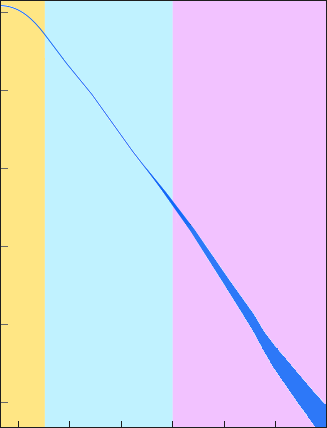
\includegraphics[width=.45\textwidth]{cosmics}};
 
    % Y-Axis
    \draw (-2.25,-2.85 ) node[anchor=east, inner sep=1em] {$10^{-27}$};
    \draw (-2.25,-1.7  ) node[anchor=east, inner sep=1em] {$10^{-21}$};
    \draw (-2.25,-.45  ) node[anchor=east, inner sep=1em] {$10^{-15}$};
    \draw (-2.25, .7   ) node[anchor=east, inner sep=1em] {$10^{-9}$};
    \draw (-2.25,1.95  ) node[anchor=east, inner sep=1em] {$10^{-3}$};
    \draw (-2.25,3.1   ) node[anchor=east, inner sep=1em] {$10^{3}$};
 
    \node[label={[label distance=0.5cm,text depth=-1ex,rotate=90]above:$F \quad (m^{-2} \text{sr}^{-1} s^{-1} \text{GeV}^{-1})$}] at (-3.1,0) {};
 
    % X-Axis
    \draw (-2.3,-2.8) node[anchor=north, inner sep=1em] {$10^0$};
    \draw (-1.5,-2.8) node[anchor=north, inner sep=1em] {$10^2$};
    \draw (- .7,-2.8) node[anchor=north, inner sep=1em] {$10^4$};
    \draw (  .1,-2.8) node[ anchor=north, inner sep=1em] {$10^6$};
    \draw (  .9,-2.8) node[  anchor=north, inner sep=1em] {$10^8$};
    \draw ( 1.7,-2.8) node[ anchor=north, inner sep=1em] {$10^{10}$};
    \draw ( 2.5,-2.8) node[ anchor=north, inner sep=1em] {$10^{12}$};
    
    % Label
    \draw (.1,-3.6) node[anchor=north, black] {$E \quad (\text{GeV})$};
  \end{tikzpicture}
  }
  \caption{%
    This plots displays the flux of cosmic rays in dependency of the particle's energy.
    The colored regions denote the particle fluxes:
    $1 \text{m}^{-2}\text{s}^{-1}$ (yellow),
    $1 \text{m}^{-2}\text{yr}^{-1}$ (cyan),
    $1 \text{km}^{-2}\text{yr}^{-1}$ (magenta).
  }
  \label{fig:cosmics}
\end{figure}

Using balloon-borne and space-based experiments the energy spectrum and components of \gls{cr} have been studied\cite{Maestro:2015lla}.
The most abundant components of cosmic radiation are protons and helium nuclei.
Elements of atomic number greater than \ce{Fe} are extremely rare.

\begin{figure}
  \centering
  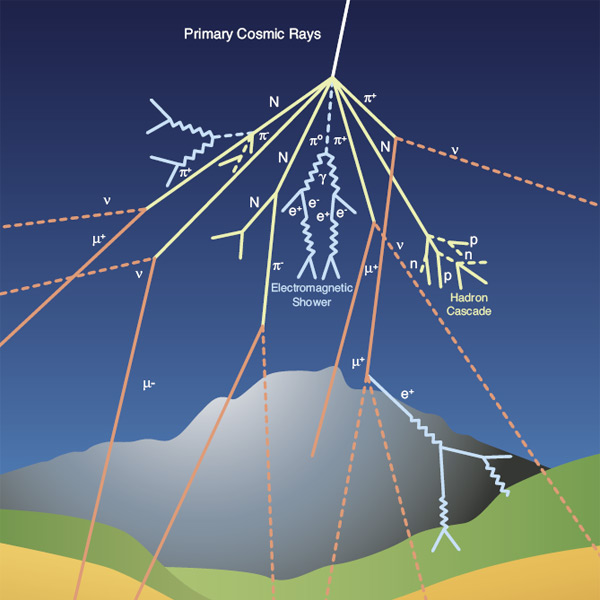
\includegraphics[width=.9\textwidth]{cosmic_ray}
  \caption{%
    A primary cosmic ray interacts in the atmosphere and produces a shower of particles as illustrated.
  }
  \label{fig:particle_shower}
\end{figure}

Cosmics contribute to the neutrino signal, due to the production of electromagnetic and hadronic showers of the constituents of the primary and subsequent cosmic rays.
Electromagnetic showers involve many photons which can contribute to the neutrino signal.
Hadronic showers result in neutral pions, which decay to high energy photons shortly after production.

\subsection{Interactions contributing to the neutrino signal}

Besides of the backgrounds contributed by the neutrino fluxes discussed in the section on neutrino sources, signal contributions of the high energy photons in these showers need to be taken into account.

The main contributions to the neutrino signal are given by compton scattering events and electron positron production.
Photons are not visible in the \gls{lartpc}'s signal, the resulting free electrons from the photon interactions cannot be distinguished from a free electron of a neutrino interaction.
See figure \ref{fig:cosmics_interactions} for an illustration.
\begin{figure}
  \centering
  \vspace{1em}
  \begin{fmffile}{sc}
    \begin{fmfgraph*}(135,100)
      \fmfleft{i1}
      \fmfright{o1,o2}
      \fmf{photon}{i1,v1,o1}
      \fmf{fermion}{v1,o2}
      \fmflabel{$\gamma$}{i1}
      \fmflabel{$\gamma$}{o1}
      \fmflabel{$e^-$}{o2}
    \end{fmfgraph*}
    \hspace*{2em}
    \begin{fmfgraph*}(135,100)
      \fmfleft{i1}
      \fmfright{o1,o2,o3}
      \fmf{phantom}{i1,v1,v2,o1}
      \fmf{photon}{i1,v1}
      \fmf{fermion}{v2,v1,o1}
      \fmf{photon}{v2,o2}
      \fmf{photon}{v2,o3}
      \fmflabel{$\gamma$}{i1}
      \fmflabel{$\gamma$}{o2}
      \fmflabel{$\gamma$}{o3}
      \fmflabel{$e^-$}{o1}
    \end{fmfgraph*}
  \end{fmffile}

  \caption{%
    Compton scattering is displayed on the left.
    Pair production with subsequent annihilation of the positrion with an electron of the medium is displayed on the right.
  }
  \label{fig:cosmics_interactions}
  \vspace{1em}
\end{figure}

The contribution of Compton scattered electrons to the electron neutino signal is comprehensible.
In the case of electron-positron pair production, the subsequent annihilation of the positron with an electron in the medium is required, to interpret the event as a neutrino interaction.


